% !TEX program = xelatex
\documentclass[UTF8,a4paper]{ctexart}
\usepackage{geometry}
\usepackage{amsmath}
\usepackage{booktabs}
\usepackage{tabularx}
\usepackage{multirow}
\usepackage{enumitem}
\usepackage{hyperref}
\usepackage{graphicx}
\usepackage{subcaption}
\usepackage{listings}
\usepackage{xcolor}
\geometry{margin=2.5cm}
\hypersetup{colorlinks=true,linkcolor=blue,urlcolor=blue}
\ctexset{
  section = {
    format = \Large\bfseries\raggedright
  },
  subsection = {
    format = \large\bfseries\raggedright
  }
}

\lstset{
  basicstyle=\ttfamily\small,
  breaklines=true,
  frame=single,
  language=Python,
  xleftmargin=1.5em,
}

% 图片统一宽度，避免单图占满整页
\newcommand{\figw}{0.66\textwidth}

\title{AI Racer 视觉自动驾驶控制器}
\author{\textit{}}
\date{}

\begin{document}
\pagestyle{plain}
\maketitle

\begin{abstract}
本项目实现了一个纯视觉、无地图、无车速反馈的 AI Racer 控制器。平台每帧传入左右双目图像与时间戳，控制器返回转向和速度两个标量。控制器采用单向四级流水线：perception 从双目图像中提取道路观测，estimator 把观测转成几何状态，policy 据此计算转向和速度，clamp 负责最终限幅。控制器按场次拆成两个隔离的 profile（参数档）：no\_other\_cars 面向单车计时，with\_other\_cars 面向多车竞速。

单车在 complex 赛道完整跑完一圈，total\_time（总用时）为 252.863\,s、best\_lap（最佳圈时）为 252.928\,s，全程零丢线、零硬撞，指令均速 0.85，满速帧（speed，速度指令 $\geq 0.95$）占 47.5\%，低速爬行帧占 0.3\%。多车评测用同一套控制器同时驱动六辆车，名次主要由发车位置决定，本报告只评价避让算法：有对手扎堆时，早避让把本车陷入车堆的帧占比从 18.5\% 压到 0.7\%，丢线率从 13\% 压到零，均速从 0.67 回到 0.85；分层脱困把最长卡死时间从十几秒压到约 2\,s，六车场景稳定完赛、零 DQ（取消资格）、零严重碰撞。开发共经历七个阶段（R001 到 R071），“转弯半径太小”贯穿前中期；最终通过定位真因、删掉错误分叉、引入速度耦合和弯中保持，把均速从 0.62 提到 0.85。
\end{abstract}

\section{任务背景与赛制}

AI Racer 平台每帧调用控制函数：
\begin{center}
\path{control(left_img, right_img, timestamp)}
\end{center}
其中：
\begin{itemize}[leftmargin=2em,itemsep=0pt,topsep=0pt]
\item left\_img 和 right\_img：左右相机 BGR 图像，各 $640\times480$；
\item timestamp：仿真时间戳；
\item steering（转向指令）取值 $[-1,1]$，speed（速度指令）取值 $[0,1]$。
\end{itemize}
这个接口带来三条硬约束，并决定后续设计取舍。

第一，控制器只有视觉输入，没有地图、定位、真实车速或惯性读数。它无法直接知道当前速度、是否被障碍物顶住、上一帧指令是否让车移动，后文的画面流动卡死检测就由此产生。第二，最终提交的 \texttt{team\_controller.py} 由构建脚本把 controller 目录下的模块按固定顺序拼成一个自包含单文件，并禁用 os、sys、time、threading、open、eval 等模块以及一切调试输出；调试代码只能留在本地。第三，\texttt{control()} 的签名没有场景标志，无法在运行时判断单车计时或多车竞速，只能由构建脚本的 \texttt{--mode} 参数注入不同参数常量（见第 \ref{sec:profile} 节）。

两类场次的目标函数不同。单车只看完赛和总时间，可以直接压圈速。多车按名次给积分，第一到第四名以及第五名及以后分别得 10、7、5、3、1 分，累计三次严重碰撞会被取消资格。多车层优先保证完赛和低碰撞预算，因此加入避让、减速和脱困。我们的评测把六个车位全部填入同一套控制器（见第 \ref{sec:multicar} 节），名次几乎只反映发车位置和偶发卡死；本报告不把名次当成绩，只讨论避让算法和脱困效果。表 \ref{tab:points} 给出官方积分规则。

\begin{table}[htbp]
\centering
\caption{多车积分规则（赛制背景，非本报告的评价指标）}
\label{tab:points}
\small
\begin{tabular}{@{}cccccc@{}}
\toprule
名次 & 1 & 2 & 3 & 4 & $\geq 5$ / 未完赛 \\
\midrule
积分 & 10 & 7 & 5 & 3 & 1 \\
\bottomrule
\end{tabular}
\end{table}

\section{系统总览}

控制器的数据流是一条单向四级流水线，如图 \ref{fig:pipeline} 所示。每帧左右图像先进入 perception，输出 PerceptionObs（道路观测）；estimator 从观测估计几何状态，写入 TrackState（赛道状态）；policy 读取 TrackState 计算控制量；clamp 把结果限到合法范围再输出。每一级只读取上一级输出，不回查原始图像：走线偏了查 estimator 或 policy，看错路查 perception，问题边界清楚。

\begin{figure}[htbp]
\centering
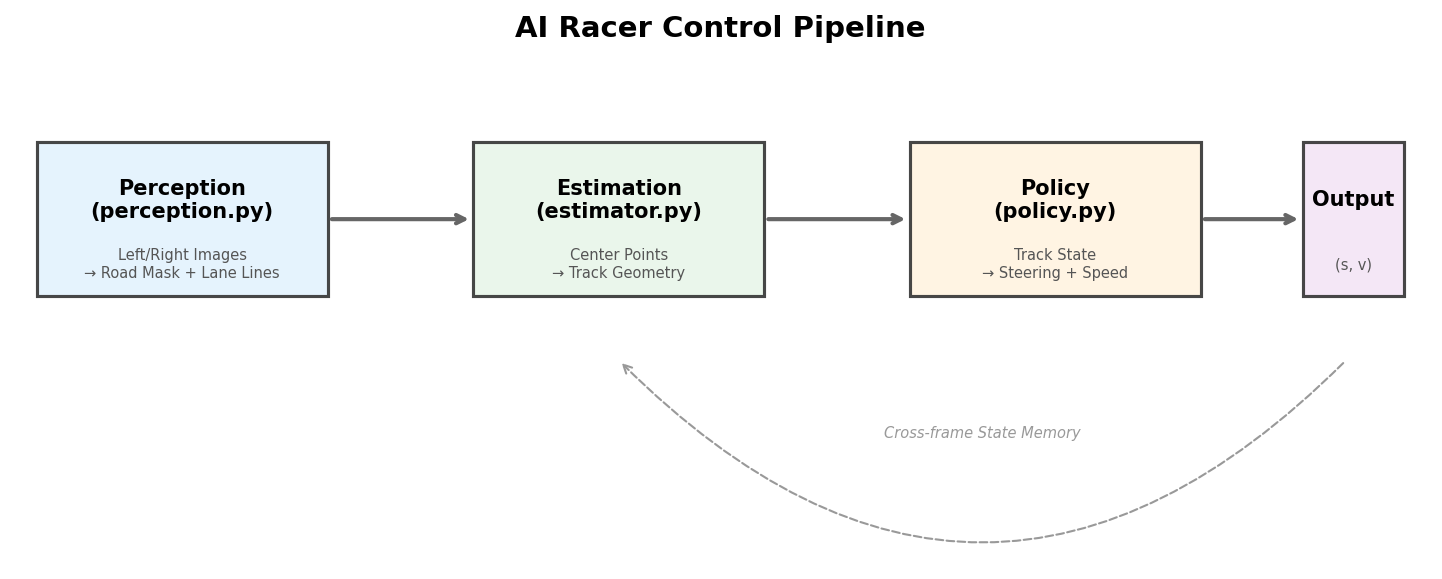
\includegraphics[width=0.82\textwidth]{../../experiments/figures/run3_analysis/fig1_pipeline.png}
\caption{四级流水线总览。四个方框自左向右依次是 perception、estimator、policy 和输出；下方那条虚线弧是跨帧状态记忆，表示入弯门控、脱困状态机、平滑器都会把本帧状态留给下一帧使用。}
\label{fig:pipeline}
\end{figure}

流水线下方还有跨帧状态记忆（图 \ref{fig:pipeline} 中的虚线弧）。入弯门控保持、脱困状态机、转向与速度平滑都读取上一帧状态，让控制器在连续帧之间保持动作连贯，避免每帧独立决策造成弯中抖动。表 \ref{tab:modules} 列出各模块职责边界。

\begin{table}[htbp]
\centering
\caption{模块职责边界}
\label{tab:modules}
\small
\begin{tabularx}{0.95\textwidth}{@{}lXX@{}}
\toprule
模块 & 负责 & 不做 \\
\midrule
perception.py & 图像处理，输出 PerceptionObs & 计算转向或速度 \\
estimator.py & 从观测估计几何状态 & 接触原图、输出控制量 \\
policy.py & 计算转向和速度 & 处理原始图像 \\
params.py & 集中存放参数 & 运行算法逻辑 \\
opponent.py & 近处车身检测 & 道路分割或控制决策 \\
team\_controller\_local.py & 接线、异常兜底、最终限幅 & 实现算法 \\
\bottomrule
\end{tabularx}
\end{table}

驾驶质量以 Webots 实跑为准，不能只看离线数字。丢线率曾多次误导判断：有一版因为蓝色场景接近天空导致道路掩膜饱和，被判成丢线，但车实际沿直线平稳滑行；也有版本把草地当路面，车朝草地开却不报丢线。每次改动都同时看实跑画面和接触日志。第 \ref{sec:backtest} 节介绍支撑这些判断的回测与诊断系统。

\section{技术实现方案}\label{sec:tech}

\subsection{感知：从双目图像到道路几何}

感知模块在没有先验地图的情况下，从单帧 BGR 图像里找可行驶区域和车道中心线。流程分三步：识别路面、追踪走廊中点、检测白色虚线。

第一步是颜色分割。我们从真实帧里采样六类颜色：深灰沥青路面、较亮路肩、蓝灰色护栏、绿色草地、红色场地、蓝色天空；每类在 HSV 和 Lab 两个色彩空间各存一组中位数和容差作为色卡。帧进来后逐像素比对色卡，命中沥青且灰度、通道差落在路面区间的像素聚成道路核心区，再扣掉草地、红场、天空和偏亮路肩。横跨赛道的蓝色检查点门颜色特殊，但门后仍是路面，因此按整行并入道路。边界条件更难处理：蓝色门和蓝色天空容易混淆，一旦天空进了路面掩膜，扫描线会把天空当成可行驶区域。代码对掩膜做形态学去碎和连通域过滤，只保留足够大、位置合理的连通块；边缘掩膜单独保留，只在道路掩膜失败时兜底。

第二步是沿扫描线追走廊。感兴趣区域内布置若干水平扫描行，从近到远逐行在道路掩膜内取连续区间中点，作为该行的道路中心候选；相邻行中点跳变过大时丢弃该点。当道路在远处分叉、或被对手车遮挡而出现多个候选段时，用上一帧保存的道路中心作为时间锚点，取与上帧最接近的候选，保持追踪的时间连续性——这在 complex 赛道 CP3 区域（多段道路在画面里合并）尤其关键。输出包括左右相机各自的道路中心点序列，以及对应的左右边界点。

第三步是白线检测。白色虚线标出车道中心，通常比走廊中点可靠：弯道内侧草地常比外侧窄，掩膜走廊中点会偏向内侧，白线不会。白线必须同时满足三项条件：足够亮、色度接近中性白、左右紧邻都是深灰路面；第三项用于排除偏蓝灰的护栏支柱和外侧路牙。检测后输出 line\_offset（白线相对车中轴的横向偏移，正值表示白线在车右侧）、line\_heading（白线走向）和 line\_confidence（按命中点数计算的置信度）。图 \ref{fig:perception} 展示一个急左弯的感知结果：青色横线是扫描行，黄色框是白线候选，红点是每行道路中心；急弯中仍能得到连续中心点和白线点。左右两目的检测在感知阶段独立完成，estimator 再按白线置信度和道路点数量融合。

\begin{figure}[htbp]
\centering
\includegraphics[width=0.82\textwidth]{../../experiments/figures/R042_to_R049_turn_in_evolution/r049_first_left_overlay.png}
\caption{R049 第一个急左弯中段的双目感知叠加图。左右两幅为左右相机，红点是逐行道路中心，黄框是白线候选；急弯里仍有连续的中心点和白线点支撑转向。}
\label{fig:perception}
\end{figure}

\subsection{几何估计：从离散点到连续状态}

estimator 把感知输出的离散点转成四个连续标量，供 policy 使用。lateral\_error（近处横偏）表示车相对近处道路中心偏左还是偏右；lookahead\_error（远处预瞄横偏）表示前方道路中心位置；heading\_error（道路走向误差）表示道路方向；curvature（曲率）表示弯的急缓。计算时先归一化中心点，再做多项式拟合：点够多时用二次拟合，否则退化为直线；近端中位数作为横偏，远端中位数作为预瞄，拟合导数作为走向，二次项作为曲率。白线置信度大于零时，按信任权重把横偏、走向和预瞄拉向白线目标，让车道中心优先于掩膜走廊中点。

curvature\_trust（曲率可信度）用于压制不可靠二次项。扫描点太少、纵向跨度不足或拟合残差偏大时，二次项多半是噪声，代码把 curvature 平滑收向零，避免远处稀疏点制造假弯。入弯门控只使用 lateral\_error 作为判据，原因在下一节展开。

\subsection{控制策略：从几何状态到转向与速度}

控制策略采用“风险分量加状态机”的结构。它从几何状态拆出曲率风险、横偏风险、置信风险、丢线风险和余量风险，合成综合风险，供速度和模式共用；再用带迟滞的五态状态机在巡航、入弯、修正、恢复、丢线之间切换。巡航对应直道并允许满速，入弯对应高曲率并允许大舵角，修正对应中等横偏，恢复用于丢线后的缓冲，丢线状态按上一帧朝向保守滑行。

目标舵角由两项构成：一项是近处回中项，按 lateral\_error 乘增益，把车拉回当前道路中心；另一项是远处预瞄项，由预瞄横偏、走向和曲率三者加权，让车提前为前方的弯做准备。两项的权重随状态和入弯门控动态调整。

入弯门控直接决定转弯半径。远处预瞄项会在车尚未到达弯口时起作用：直道后段已经看见前方弯道时，预瞄项会提前向弯内侧打方向，造成切内线。门控用连续乘子控制远处预瞄项释放时机，让车先沿线开到弯口，横偏出现后再加大转向。这个乘子叫 corner\_arrival（入弯到达度），只看近处横偏绝对值：直道上车居中、横偏接近零，乘子接近零，远处预瞄项被压住；车到弯口后向外漂，横偏变大，乘子升高并释放预瞄项。turn\_in\_lateral\_ref（入弯横偏基准，当前 0.75）负责归一化，调小会更早转、半径更小。

这套门控有三处设计。第一，判据只用近处横偏，不用走向或远处曲率；后两者在直道接近段就可能偏大，用作判据会提前开门。入弯瞬间，远景弯道尚未展开，也无法可靠判断弯的急缓。第二，门控与速度耦合：车速越高，横偏长起来前已经多跑了一段距离，因此高速时按 turn\_in\_speed\_comp（入弯速度补偿，当前 0.6）收小有效基准，让门提前开。第三，门控带保持与出弯迟滞：横偏在弯中会短暂回落，若不保持，远处预瞄项会被收掉，车容易转到一半就收轮；进弯后把乘子锁到峰值，出弯时按 turn\_in\_hold\_decay（入弯保持衰减，当前 0.92）逐步松开。第 \ref{sec:explore} 节深挖 A 给出这些设计的演进证据。

门控之外还有白线减预瞄。当可信白线显示车已经骑到内侧（line\_offset 与远处项反号）时，按内侧程度和置信度成比例削弱远处预瞄项，并带迟滞保持，用来打断弯中切内、往外打、过头后再次切内的振荡。它只缩远处转向项，不改风险和速度。转向输出还会经过按模式的指数平滑、逐帧变化率限制和高速收舵。速度以基准速度为底，乘上弯道、横偏、置信、转向等降速因子；curve\_power（曲率降速指数，当前 1.5）控制曲率到速度的映射；单帧加速幅度设有上限，避免丢线恢复后突然窜出。最后的后置白线修正只小幅调整输出舵角，不进入风险、速度或门控。

\subsection{多车层}

多车层只在 with\_other\_cars 这个 profile 中启用，在单车驾驶底座上叠加对手感知、避让和脱困三类能力，由 enable\_opponent（对手逻辑总开关）控制。

感知端由 opponent.py 负责。它在画面下半部中间的检测区并行寻找三类车身候选：亮白区域、近黑区域和高饱和官方彩色车身；低饱和色卡被跳过，因为容差太宽，会把 complex 的深灰沥青路面误吃成车身，这也是第 \ref{sec:explore} 节深挖 B 中一次误检的来源。候选经形态学去碎和连通域过滤后取最大块，输出三项：是否有近处对手、对手在画面里的横向位置（左负右正）和对手块尺度（越大通常越近）。frame\_motion（画面流动量）取相邻帧下采样灰度图的平均绝对差，用于判断画面是否还在移动。实测标定显示，正常行驶时 frame\_motion 不低于 0.47、中位约 0.81，被顶住空转时约 0.07，差异足以触发卡死判断。

策略端的避让分两步。第一步是减速：检测到近处对手时按其居中程度分档减速，正前方挡路的车减得多，偏在一侧的车减得轻，避免一被超车就长期缩在后面；如果同时正在弯中，还会再叠一层减速以防多车在弯里相撞卡死。第二步是有界转向偏置：朝边界余量更大的开阔一侧加一个偏置绕行，并按对手的横向位置朝其反侧让开，整个偏置被钳在一个上限内，和后置白线修正一样只改最终舵角、不进风险和速度。

脱困是一条按优先级排列的四层自救链，如图 \ref{fig:escape} 所示。最上层的顶栏脱困处理车身斜着楔进栏杆的情形：反方向大舵角做三点掉头，先倒车拉开距离，再前冲。第二层的边界障碍脱困处理一侧被静态物顶住的情形：朝开阔侧打舵，低速挪出。第三层的低速失速脱困在指令速度持续接近零时触发：前轮按方波左右摆动（在 0.95 上叠加正负 0.30、每十帧翻向一次，见图下半），借摆动打破静摩擦。最底层是 force\_escape（强制脱困安全网），由三个触发器任一激活：持续丢线、指令速度长时间接近零、画面几乎不动但指令仍在前进。最后一项就是光流卡死检测，它在无车速反馈时识别“撞栏顶住但控制器仍以为在巡航”的情况。安全网激活后先朝开阔侧净倒一段，把车从车堆里倒出来，再前冲脱离。

\begin{figure}[htbp]
\centering
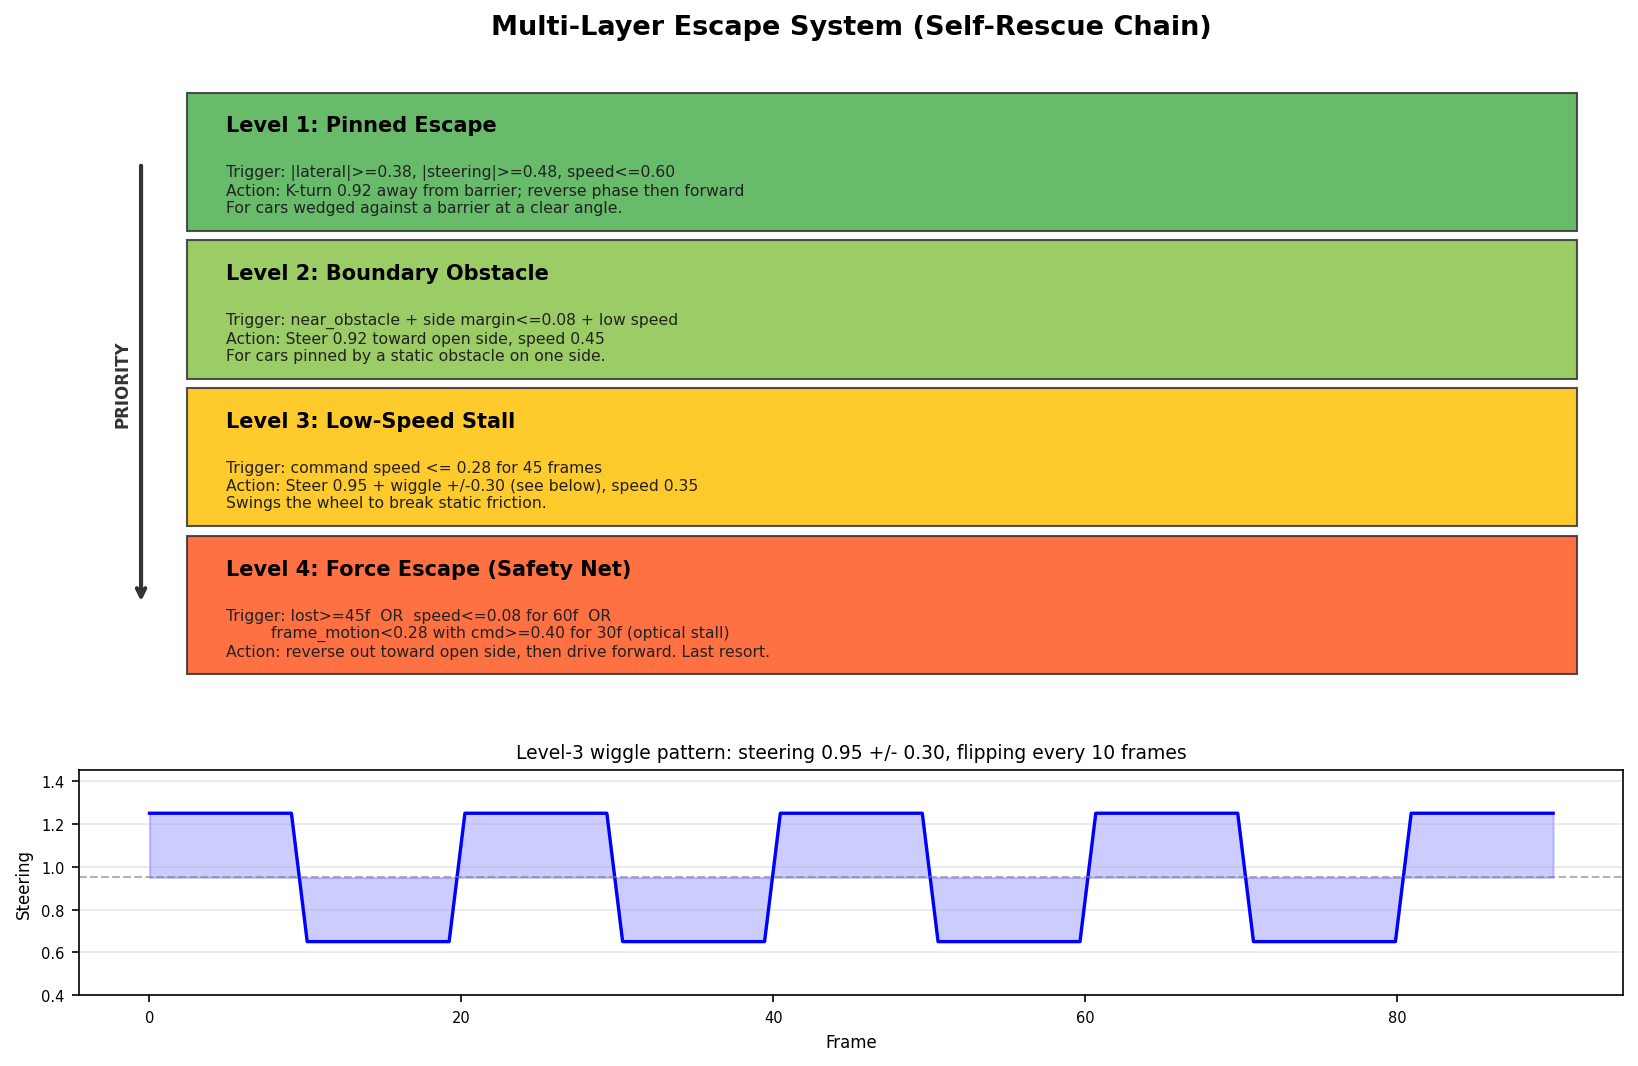
\includegraphics[width=0.86\textwidth]{../../experiments/figures/run3_analysis/fig3_escape.png}
\caption{四层脱困自救链按优先级排列（上为最先评估的高优先层），每层标注触发条件与动作；下方子图是第三层的方波摆动示意：转向在 0.95 上下摆动正负 0.30、每十帧翻向一次。}
\label{fig:escape}
\end{figure}

倒车存在一个线上线下差异。受困时控制器把速度设成负值让车后退，本地 Webots Driver 接口会真倒车；线上沙箱会把速度钳回 $[0,1]$，负值退化成原地停顿。因此脱困逻辑保留前进相位作为线上兜底：倒车线下有效，线上退化但不致命。

\subsection{Profile 隔离}\label{sec:profile}

Profile 隔离来自一次污染事故（见第 \ref{sec:explore} 节深挖 B）。接口不区分单车和多车，只能在构建层和运行层做隔离。

参数层面，单车参数字典从多车字典派生，共享入弯门控、速度、曲率等驾驶参数，只覆盖两类键：脱困参数改用更保守的值，所有多车增量参数置为禁用，包括 enable\_opponent。运行层面，当前 profile 贯穿整条流水线：perception 每帧根据开关决定是否运行对手检测和 frame\_motion；单车下两者都不运行，是否有对手恒为假，对手位置和尺度恒为零，frame\_motion 保持默认高值，卡死检测永不触发；policy 里的 force\_escape 和卡死触发也用同一个开关再守一道。单车直接跳过多车代码路径，同时每帧省下约 5\,ms 检测开销。test\_profile\_isolation.py 锁定这条约束。

\section{程序代码说明}\label{sec:code}

本节从代码组织的角度补充说明：各文件如何分工、关键算法落在哪些函数里、模块之间靠什么数据结构通信，以及提交文件如何构建和校验。算法本身的设计动机已在第 \ref{sec:tech} 节展开，这里不再重复，只把它落到文件和函数上。

\subsection{文件组织与模块分工}

代码集中在 controller/ 目录，每个文件单一职责，按数据流串成一条单向流水线，职责边界见前文表 \ref{tab:modules}。common.py 定义三个数据契约和限幅函数，是模块间的通信基础。params.py 把所有可调参数集中存放，并按场次派生出 no\_other\_cars 与 with\_other\_cars 两套常量字典，由 get\_profile 按名分发。perception.py 负责颜色分割、扫描线追走廊和白线检测，对外入口是 extract\_observation，内部由 \_build\_masks、\_scan\_image、\_camera\_line\_state、\_fuse\_scans 等函数分别完成掩膜生成、逐行扫描、白线提取和左右融合。estimator.py 把离散点拟合成连续几何状态，入口是 estimate\_track。policy.py 是控制核心，入口 decide\_control 依次调用 \_control\_signals（风险分量）、\_select\_mode（状态机）、\_target\_steering（含入弯门控）、\_target\_speed（限速）和 \_escape\_if\_stalled（脱困）。opponent.py 只做近处车身检测，入口 detect\_near\_vehicle\_obstacle\_state，仅在多车 profile 下被调用。team\_controller\_local.py 是平台入口，只做接线、异常兜底和最终限幅，不含算法。

这种按文件划清职责的方式，使每个问题都能定位到唯一的文件：走线问题查 estimator 或 policy，看错路查 perception，参数问题查 params，对手相关查 opponent。它也是单向流水线得以维持、改一处不至于牵动全局的前提。

\subsection{关键数据结构}

三个 dataclass 构成模块间的通信契约，都定义在 common.py，主要字段见表 \ref{tab:datastruct}。它们是硬契约：改动任一字段，都必须同步全部调用方、构建脚本和测试，否则拼接出的单文件会在运行时出错。

\begin{table}[htbp]
\centering
\caption{模块间的三个数据契约（common.py）}
\label{tab:datastruct}
\small
\begin{tabularx}{0.97\textwidth}{@{}llX@{}}
\toprule
数据结构 & 主要字段 & 含义 \\
\midrule
\multirow{4}{*}{\shortstack[l]{PerceptionObs\\（感知输出）}}
 & center\_points / left\_edge\_points / right\_edge\_points & 逐行道路中心点与左右边界点 \\
 & road\_width\_est, confidence & 道路宽度估计、感知置信度 \\
 & line\_offset / line\_heading / line\_confidence & 白线偏移 / 走向 / 置信度 \\
 & near\_obstacle / obstacle\_x / obstacle\_size / frame\_motion & 近处对手标志 / 横向位置 / 尺度 / 画面流动量 \\
\midrule
\multirow{3}{*}{\shortstack[l]{TrackState\\（几何状态）}}
 & lateral\_error / lookahead\_error & 近处横偏 / 远处预瞄横偏 \\
 & heading\_error / curvature & 道路走向 / 曲率 \\
 & confidence / lost / red\_environment & 置信度 / 丢线标志 / 红色场地标志（其余为感知透传） \\
\midrule
ControlCmd（控制命令） & steering / speed & 转向 / 速度指令 \\
\bottomrule
\end{tabularx}
\end{table}

TrackState 除了五个核心几何量，还把白线、边界余量、对手和画面流动等字段从 PerceptionObs 透传给策略，使 policy 不必回读原图。ControlCmd 只有转向和速度两项；入口层用 clamp\_cmd 做最终限幅，其中转向钳到 $[-1,1]$、速度下界被放宽到 $-1.0$ 以支持倒车脱困，而线上沙箱会再把速度钳回 $[0,1]$。

\subsection{构建、提交与测试}

提交文件由 build\_submission.py 生成，它按 common、params、opponent、perception、estimator、policy、team\_controller\_local 的固定顺序把各模块拼成一个自包含的 team\_controller.py，过程中自动删去本地 import 语句和一切调试输出（open、json、cv2.imwrite 等），并用 \texttt{--mode} 注入对应 profile 的参数。带调试输出的版本用 \texttt{--debug-log} 和 \texttt{--dump-frames} 构建，只在本地使用、绝不上传。校验分两层：validate\_submission.py 检查接口契约、静态规则和 mock 图像下的输出范围，官方 validate\_controller.py 做更严格的沙箱合规检查。仓库的 pytest 共 149 个用例，覆盖感知 dropout、白线跟踪、入弯门控、脱困、输出范围以及 profile 隔离等关键路径。

\section{回测与诊断系统}\label{sec:backtest}

控制器拿不到真值，平台默认看不见撞栏，离线数字也会误导判断。只改代码再上传看结果，无法判断改动到底改善了什么。我们围绕 Webots 搭了一套回测流程，覆盖自动实跑、自动取证和量化判读。下面按问题说明各工具。

第一项是一键实跑与产物归档。webots\_run.sh 自动构建带调试输出的控制器、清理残留 Webots 进程、跑完整场，并默认每十帧保存一对无损左右相机帧。跑完后，任意时刻的画面都能事后翻看，不必为了看某一帧重跑两百多秒。脚本默认开启撞栏接触日志，每场结束后滚动归档上一轮产物，保留最近十轮。后续取证都依赖这批可复盘产物。

第二项是无人值守多车自跑。webots\_auto\_multicar.sh 带看门狗，在后台启动六车 Webots；超时或日志长时间不动时自动收尾；车数、最大时长、静止判定秒数、对手速度缩放都可配置。对手速度缩放小于一时，会得到对手统一变慢的纯超车测试场景，用来检验本车能否干净追上并超过慢车。改代码、自动跑、读日志的循环因此可以无人值守执行。

第三项是世界状态跳转，用来降低复现成本。早期复现某个弯或卡点，常要从发车格重跑两百多秒。webots\_jump\_run.sh 配合 make\_teleport\_world.py，可以从历史遥测里取出某一时刻的位姿（坐标和朝向），临时生成一个让车直接出生在该位置的世界。观察“当前代码从这个姿态会怎么开”从分钟级降到秒级。它只恢复位姿、不恢复速度，属于近似续跑，但足够验证走线想法。

第四项是撞击、位置和速度检测，用来补上平台看不见撞栏的空白。我们在 SDK 的 supervisor 层注入接触检测，由环境变量开关控制，只在本地生效；它逐帧记录车身与栏杆、静态几何体的接触，输出结构化日志，字段包括时间、世界坐标、接触点数和最大穿透深度。判读规则来自大量实跑标定：同一窗口内接触点数峰值不少于三，且最大穿透深度超过 0.6，判为真撞栏；孤立一两点，或穿透深度落在发车格路面的固定阈值附近，判为底盘伪接触。多车场景还要按车位过滤，否则会把对手撞栏误算到本车头上。位置、速度、近停和事件由遥测日志配合分析脚本给出。这样离线分析也能定位每次撞栏的时间、位置和严重程度。

第五项是逐帧视觉识别标注，用来回答某一帧里控制器到底看到了什么。对应脚本是：
\begin{center}
\path{analyze_perception_dump.py}
\end{center}
它读取已保存的相机帧和控制日志，在指定时刻把感知中间结果画回画面：道路掩膜、边缘、扫描线、逐行道路中心红点、白线候选黄框，并标注走廊填充率和道路点数。图 \ref{fig:perception} 的弯道叠加图和图 \ref{fig:residual} 的残留窗口图都来自这条脚本。走线出问题时，标注图能区分是看错路，还是看对了但策略不对。

第六项是开环回放，用来判断改动是否真的生效。实跑带随机性，同一版代码两次轨迹也不完全一致，只比较两次实跑很难区分算法变化和随机差异。replay\_offline.py 把同一批已保存相机帧重新喂给当前代码，输出开环控制日志；改动前后可以在完全相同的视觉输入下逐字段比较线置信度、舵角、模式等量。许多改动是否有效，最后都靠开环回放确认。

最上层是一组量化判读脚本。内部模式脚本统计模式分布、舵角、速度和线置信度；撞栏脚本按赛段统计次数和严重程度；脱困脚本统计每次脱困持续多久、是否倒车、倒车后是否恢复、是否误触发；多车 KPI 脚本量化名次期望积分、完赛、取消资格、严重碰撞预算、超车净得失、开局挤压、卡死时长和速度。多车避让是否有效，最终看这些指标。轨迹绘图脚本把整场轨迹按速度着色并叠加撞栏点，本文的轨迹图都出自这里。

\section{当前效果与赛道成绩}

\subsection{单车计时}

单车计时全部来自 complex 赛道。这条赛道一圈约 1320\,m，含连续急弯、内环分岔、红色场地和静态障碍段。表 \ref{tab:single_time} 列出最近几次官方计时。R068 的 252.863\,s 是当前最佳；R069 与 R071 是清理性能软警告 W014 前后的同环境对照，结果完全一致（254.495\,s），说明那次清理没有改变驾驶行为。

\begin{table}[htbp]
\centering
\caption{单车计时成绩（complex，no\_other\_cars）}
\label{tab:single_time}
\small
\begin{tabular}{@{}cccc@{}}
\toprule
Run & total\_time (s) & best\_lap (s) & 严重碰撞 \\
\midrule
R067 & 254.495 & 254.560 & 0 \\
R068 & \textbf{252.863} & \textbf{252.928} & 0 \\
R069 & 254.495 & 254.560 & 0 \\
R071 & 254.495 & 254.560 & 0 \\
\bottomrule
\end{tabular}
\end{table}

圈时之外，还需要看驾驶质量。表 \ref{tab:driving_quality} 使用 R049 的控制日志（8053 帧、257.7\,s）做统计：丢线率为零，满速帧（speed $\geq 0.95$）占 47.5\%，低速爬行帧只有 0.3\%。早期弯中掉速到零、再慢慢爬出的现象基本消失。图 \ref{fig:r049_traj} 的顶视图也显示，整条赛道大部分轨迹是高速对应的暖色，只有弯心转冷；速度曲线进弯规律回落、出弯快速回升。整场只有七处轻微接触，接触点峰值不超过三、穿透深度不超过 0.50，没有硬撞。

\begin{table}[htbp]
\centering
\caption{R049 单车驾驶质量（8053 帧 / 257.7\,s，来自控制日志）}
\label{tab:driving_quality}
\small
\begin{tabular}{@{}lr@{}}
\toprule
指标 & 数值 \\
\midrule
丢线率 & 0.0\% \\
指令均速 / 中位速度 & 0.85 / 0.893 \\
满速率（speed $\geq 0.95$） & 47.5\% \\
高速率（speed $\geq 0.85$） & 56.4\% \\
低速爬行帧（speed<0.45） & 0.3\% \\
模式占比（巡航 / 入弯） & 55\% / 45\% \\
\bottomrule
\end{tabular}
\end{table}

图 \ref{fig:speed_dist} 的速度直方图和表 \ref{tab:speed_bucket} 的曲率风险分桶显示，直道均速 0.95，中低曲率弯 0.91，中高曲率弯 0.82，急弯 0.66，帧数主要落在直道和中等弯。curve\_power 提到 1.5 后，直道和中等弯保留速度，接近物理极限的急弯才明显降速。

\begin{figure}[htbp]
\centering
\includegraphics[width=0.60\textwidth]{../../experiments/figures/R045_to_R049_speed_evolution/r049_trajectory_speed_contact.png}
\caption{R049 整场顶视轨迹（按速度着色）与速度曲线。行驶距离 1320.4\,m，末态正常；暖色为高速、冷色为弯心低速，深色点为七处轻微接触。}
\label{fig:r049_traj}
\end{figure}

\begin{figure}[htbp]
\centering
\includegraphics[width=0.70\textwidth]{../../experiments/figures/R045_to_R049_speed_evolution/r049_speed_distribution.png}
\caption{R049 指令速度直方图与按曲率风险分桶的均速。}
\label{fig:speed_dist}
\end{figure}

\begin{table}[htbp]
\centering
\caption{R049 按曲率风险分桶的均速（来自控制日志）}
\label{tab:speed_bucket}
\small
\begin{tabular}{@{}lrr@{}}
\toprule
曲率风险区间 & 均速 & 帧数占比 \\
\midrule
直道（< 0.10） & 0.950 & 38.3\% \\
中低（0.10--0.30） & 0.912 & 17.6\% \\
中高（0.30--0.55） & 0.816 & 22.4\% \\
急弯（> 0.55） & 0.657 & 21.6\% \\
\bottomrule
\end{tabular}
\end{table}

\subsection{多车避让算法的实现与效果}\label{sec:multicar}

多车测试用同一套 with\_other\_cars 控制器同时驱动全部六个车位，各车名次差异几乎只反映发车位置和偶发卡死，不能说明策略优劣。本节只验证避让算法：有对手的拥挤环境里，本车能否避免被卡死、能否穿出车堆、能否超过更慢的车。图 \ref{fig:multicar_pos} 是同策略六车场的位置快照。发车时六车挤在格内并互有轻触；比赛中后段，多辆车相继卡死（图中红色 STUCK 标注）；本车（红圈）始终推进，完赛后停在格内。这就是避让和脱困层要处理的环境。

\begin{figure}[htbp]
\centering
\includegraphics[width=0.74\textwidth]{../../experiments/figures/run3_analysis/fig4_multicar_positions.png}
\caption{同策略六车在四个时刻的位置快照，红圈为本车。多辆对手在中后段相继卡死（红色 STUCK），本车始终在推进。此图用于展示拥挤环境，不用于比较名次。}
\label{fig:multicar_pos}
\end{figure}

避让效果用受控测试量化，结果见表 \ref{tab:avoid_effect}。第一组对照发生在弯道附近对手扎堆的窗口：无避让版本会扎进车堆，视角被对手车身挡住，脱困状态帧占 18.5\%，丢线率 13\%，均速掉到 0.67；加入早避让后，本车绕开并超过卡死的对手堆，脱困帧降到 0.7\%，丢线率归零，均速回到 0.85。第二组是纯超车测试：对手统一降速到 0.55，本车全速追上并超过，均速 0.85、中位 0.92、丢线率为零、全程零倒车，接触只有发车格轻触。减速和有界绕行把本车从被夹住改成了能穿过去。

\begin{table}[htbp]
\centering
\caption{多车避让 / 超车的受控测试效果}
\label{tab:avoid_effect}
\small
\begin{tabularx}{0.96\textwidth}{@{}Xlrrrl@{}}
\toprule
场景 & 设置 & 脱困帧占比 & 丢线率 & 均速 & 结果 \\
\midrule
穿越对手车堆 & 无避让 & 18.5\% & 13\% & 0.67 & 扎进车堆被糊住 \\
穿越对手车堆 & 早避让 & 0.7\% & 0\% & 0.85 & 绕开并超过 \\
追超更慢的车 & 对手降速 0.55 & --- & 0\% & 0.85（中位 0.92） & 干净超车，零倒车 \\
\bottomrule
\end{tabularx}
\end{table}

脱困层主要压缩卡死时间。图 \ref{fig:escape_iter} 对比三轮迭代：最初没有摆动，弯里遇到对手只会减速，卡死十七秒，整场失败；加入方波摆动和零速检测后，卡死缩到十一秒，但仍然失败；再加入弯道减速，把摆动幅度定到 0.30，并提高触发灵敏度后，最长卡死约两秒，整场跑满两百七十多秒。配合光流卡死检测和倒车相位，贴边空转、车堆顶停这类刚性陷阱可以自救恢复。六车场景稳定完赛、零取消资格、零严重碰撞：避让减少卷入车堆，脱困处理偶发受困。

\begin{figure}[htbp]
\centering
\includegraphics[width=0.66\textwidth]{../../experiments/figures/run3_analysis/fig5_run_comparison.png}
\caption{脱困逻辑三轮迭代的卡死时间对比。前两轮整场失败、最长卡死十七秒与十一秒；第三轮跑满两百七十多秒、最长卡死约两秒。}
\label{fig:escape_iter}
\end{figure}

\section{探索过程}\label{sec:explore}

开发经历七个阶段。Stage 0（R001--010）搭起基础驱动和感知基线，确定丢线滑行加低速脱困方案。Stage 1（R011--025）进入 complex 赛道，引入白线优先策略，完成从 basic 到 complex 的感知迁移；basic 椭圆赛道在此阶段先实现了稳定的物理完赛（一圈约 288\,s）。Stage 2（R026--038）首轮处理转弯半径，把车从早切内、撞栏推进到能完整跑一圈，但半径仍偏小。Stage 3（R039--049）系统重做入弯门控，是下面深挖 A 的主线。Stage 4（R050--052）搭起多车基础策略并验证六车跑通。Stage 5（R053--061）完成多车脱困、避让和卡死检测，期间发生一次 profile 污染事故，即深挖 B。Stage 6（R062--071）建设度量基建、拆分 profile、修好官方完赛与名次统计，并完成性能清理。

七个阶段反复验证了一条经验：保守微调几乎没用。从 R026 到 R049 的转弯半径攻坚中，有效改动都发生在机制层面，包括更换入弯判据来源、改变门控形状、改变速度耦合方式；在同一套逻辑里反复拧参数，大多只是换一种方式暴露问题。

\subsection{深挖 A：转弯半径太小的解决}

转弯半径太小贯穿 R026 到 R049。最初表现为急弯切向内栏并撞上去，部分弯后还会长时间掉速爬行（图 \ref{fig:r026r038} 左）。R038 已能完整跑过一圈（图 \ref{fig:r026r038} 右），但仍贴内线、轻擦内栏。R041 到 R049 完成诊断和修复。

\begin{figure}[htbp]
\centering
\begin{subfigure}{0.49\textwidth}
\centering
\includegraphics[width=\textwidth]{../../experiments/figures/R026_first_left_tight_radius/trajectory_speed.png}
\caption{R026：第一个左弯掉速到零、长时间爬行，未完赛。}
\end{subfigure}\hfill
\begin{subfigure}{0.49\textwidth}
\centering
\includegraphics[width=\textwidth]{../../experiments/figures/R038_best_human_residual_tight_radius/trajectory_speed.png}
\caption{R038：已能完整跑完一圈，速度规律起伏，但残留半径偏小。}
\end{subfigure}
\caption{Stage 1 到 Stage 2 的对照：从“首左弯卡死”到“能跑完整圈但仍贴内”。}
\label{fig:r026r038}
\end{figure}

第一步是定位真因。早期入弯门控用走向和远处弯量判断是否到达弯口；走向在直道接近段就可能偏大，弯还在前方，门控已经提前释放预瞄项，车因此切进内线。图 \ref{fig:before_after} 给出同一个最紧左弯的对照。左列是旧的走向驱动门控版本（R041）：入弯发生在横偏约 $-0.01$ 时，车几乎还居中；随后舵角和线偏移剧烈振荡，线偏移反复越过 0.35 的内侧阈值，峰值达到 $+0.65$，最后十二个接触点硬撞。右列是改用横偏判据后的版本（图中标为 R044 的“横偏加弯急度门控”）：同一个弯里，舵角、横偏和线偏移几乎是一条平线，车骑线过弯，没有撞栏。对照显示，入弯太早就是切内线根因。

\begin{figure}[htbp]
\centering
\includegraphics[width=0.92\textwidth]{../../experiments/figures/R042_to_R049_turn_in_evolution/r041_r042_turn_in_before_after.png}
\caption{同一最紧左弯的入弯对照。左列（R041，走向驱动门控）在横偏约 $-0.01$、车还居中时就开始入弯，随后线偏移反复越过内侧阈值 0.35、峰值 $+0.65$，十二点硬撞；右列（改用横偏判据后）全程近乎平线、稳稳骑线。}
\label{fig:before_after}
\end{figure}

第二步是删掉错误路线。确定只用横偏之前，我们尝试按弯的急缓调门控：曲率风险低就当缓弯、晚开门；曲率风险高就当急弯、早开门。缺陷出现在入弯瞬间：弯还没在视野里展开，曲率风险往往偏低，急弯入口也会被误判成缓弯并过度延迟；车深入弯中后曲率风险才升高，门才打开，此时急打轮反而半径更大，还会冲外、掉速。R044 用这套方案后，某些弯不再切内，却出现外偏甚至蹭外侧。R046 删除这条按弯急缓分叉的逻辑，回到纯横偏门控。

第三步是看清门控形状。图 \ref{fig:gate_shape} 把三代门控画在同一张图上，横轴是横偏绝对值，纵轴是远处预瞄项放行比例。旧版（红线）在横偏为零时已经开到约 0.94，几乎一开始就放行，造成早切内。纯横偏版（蓝线）改成线性，要到横偏约 0.75 才完全放行。速度耦合版（紫线）更陡，高速下有效基准降到约 0.43 就放满，用来补偿高速时多跑出的距离。

\begin{figure}[htbp]
\centering
\includegraphics[width=0.60\textwidth]{../../experiments/figures/R042_to_R049_turn_in_evolution/turn_in_gate_shape.png}
\caption{三代入弯门控形状对比。红线（旧）横偏为零时已近全开；蓝线（纯横偏）到 0.75 才全开；紫线（速度耦合）在高速有效基准约 0.43 处全开。}
\label{fig:gate_shape}
\end{figure}

第四步是补上速度和保持。R047 把速度引入门控基准：车速越高，横偏长起来前已经多跑了一段，如果沿用低速门控，几何上同样晚，物理上更晚，表现为冲外、半径过大；高速时门必须更早开。速度在入弯瞬间已经稳定可用，比按弯急缓调制可靠。R048 给门加上跨帧保持：门开满后锁住，出弯后再慢慢松开，解决横偏在弯中短暂回落导致门塌掉、车转到一半收轮的问题。

图 \ref{fig:tight_evo} 和表 \ref{tab:tight_evo} 给出同类紧弯在四个关键版本上的指标变化：R041 线偏移峰值 0.65（严重切内）、十二点硬撞、均速 0.61；R042 线偏移峰值降到 0.23，切内和硬撞消失；R044 降到 0.02，横向几乎不动，但这一版后来因外偏被删；R049 峰值为 0.79，方向向外，不再切内，只剩轻擦，均速 0.81。这串数字对应一组机制修正，不是单次调参。

\begin{figure}[htbp]
\centering
\includegraphics[width=0.56\textwidth]{../../experiments/figures/R042_to_R049_turn_in_evolution/tight_corner_control_progression.png}
\caption{同类紧弯控制量在四个版本上的演进（自上而下 R041 / R042 / R044 / R049）。}
\label{fig:tight_evo}
\end{figure}

\begin{table}[htbp]
\centering
\caption{紧弯控制逐代演进（同一最紧弯窗口）}
\label{tab:tight_evo}
\small
\begin{tabular}{@{}lccl@{}}
\toprule
版本 & 线偏移峰值 & 均速 & 说明 \\
\midrule
R041 & 0.65 & 0.61 & 旧门控，十二点硬撞 \\
R042 & 0.23 & 0.75 & 改横偏判据，硬撞消失 \\
R044 & 0.02 & 0.95 & 按弯急缓分叉（后因外偏删除） \\
R049 & 0.79 & 0.81 & 当前最佳，峰值方向向外、仅轻擦 \\
\bottomrule
\end{tabular}
\end{table}

入弯修复同期也在提速。图 \ref{fig:speed_evo} 左展示 R044 到 R049 的均速进展：0.62 到 0.83，再到 0.85；中位速度从约 0.66 提到 0.89，丢线率始终为零。提速分四步：放开过保守的全局限速和直道速度；加入速度耦合，避免高速入弯因门控过晚而冲外；用门控保持减少弯后跑偏、再修正、再掉速的隐性损失；定向提升中等弯速度。最后一步依赖 curve\_power 这个旋钮（图 \ref{fig:speed_evo} 右）：提到 1.5 后，中等曲率弯的速度因子抬高，曲率风险到顶的急弯端点不变。急弯已经接近速度与半径的物理边界，再快会更宽甚至撞栏。

\begin{figure}[htbp]
\centering
\begin{subfigure}{0.49\textwidth}
\centering
\includegraphics[width=\textwidth]{../../experiments/figures/R045_to_R049_speed_evolution/speed_progression_r044_to_r049.png}
\caption{R044 到 R049 均速进展（0.62 → 0.83 → 0.85）。}
\end{subfigure}\hfill
\begin{subfigure}{0.49\textwidth}
\centering
\includegraphics[width=\textwidth]{../../experiments/figures/R045_to_R049_speed_evolution/curve_power_effect.png}
\caption{curve\_power 提到 1.5：只抬中等弯，急弯端点不变。}
\end{subfigure}
\caption{提速的两条证据：整体均速抬升，且通过 curve\_power 把提速集中在中等弯。}
\label{fig:speed_evo}
\end{figure}

仍有一个残留问题：两个肉眼相近的弯，走线半径可能不一致。原因不在门控，而在感知给出的曲率风险不够稳定，导致速度不同、物理半径不同。图 \ref{fig:residual} 是代表帧：这个右弯里左右相机白线点都偏少，证据稀疏，纠正偏晚，车已经落到白线内侧。这属于感知一致性问题，不是入弯门控复发。

\begin{figure}[htbp]
\centering
\includegraphics[width=0.74\textwidth]{../../experiments/figures/R038_best_human_residual_tight_radius/overlay_000226_560.png}
\caption{残留窗口的双目叠加图：白线点稀疏，纠正偏晚，车落到白线内侧。这是感知一致性问题，不是入弯门控问题。}
\label{fig:residual}
\end{figure}

\subsection{深挖 B：Profile 污染事故与隔离}

事故发生在 Stage 5 早期。当时为了做多车，把对手避让、倒车、安全网脱困和光流卡死检测直接加到唯一一套参数上，等于把多车策略强加给单车。单车计时赛里没有对手，也没有障碍，这些行为仍可能被触发：光流卡死检测会在某个急弯减速窗口误判画面不动，触发倒车和摆轮；避让逻辑也可能因画面干扰产生无谓减速和转向，拖慢单车成绩。

修复分三层。参数层拆出单车和多车两套字典，单车字典从多车派生，但把所有多车增量覆盖为禁用；运行层用总开关贯穿感知和策略，单车下不跑对手检测和画面流动计算，也不进入安全网触发；测试层用专门测试锁定硬约束：单车下没有近处对手、对手位置为零、画面流动量为默认值。这次事故的教训是，多车增量必须在单车下完全不执行，不能依赖“参数设成零所以不会触发”的软约束；参数为零时分支代码仍在运行，状态仍在累积，和其他逻辑交互后仍可能意外触发。

\subsection{深挖 C：度量不可信的根因修复}

多车迭代长期拿不到完赛圈数、进度和名次，多车目标无法度量。根因有三处。第一，supervisor 里的检查点坐标是占位值，和真实赛道检查点门对不上；车实际开过门，记录的进度不推进。第二，检查点触发门只有 0.1\,m 厚，车以约 6\,m/s 通过时，一帧位移就可能跨过整个触发区，连起跑线都会漏触发。第三，检查点初始序号错误，发车后第一次过线没有被当作计时起点，后续序号也跟着错位。修复时按真实赛道检查点门坐标重写配置，把门沿行进方向加厚到约 2.5\,m，保证至少两三帧落在门内，并修正初始序号。修好后才拿到非空完赛和名次记录，圈时、进度、碰撞预算有了可信基准。度量被验证前，基于它的优化都不可靠。

\section{不足与经验教训}

\subsection{不足与后续工作}

避让算法目前偏保守。它的策略是看到车就减速、朝开阔侧绕开，属于安全绕行；还没有基于车位、比赛阶段和相对速度做主动占位，例如卡住内线迫使对手走外线。多车方向下一步应把避让从 safe detour（安全绕行）推进到主动占位。

起步格拥挤仍未解决。图 \ref{fig:multicar_pos} 里，发车时六车在格内密集重叠并轻触；目前没有起步阶段专用分流或错峰逻辑。偶发轻触不致命，但遇到更激进的对手时可能放大成卡死。

感知一致性导致残留半径差异（图 \ref{fig:residual}）。相似弯上的曲率风险估计不稳，进而造成速度不同、物理半径不同。后续需要提高不同光照和路面下的白线点密度一致性，并重新检查曲率信任度的动态范围。

性能还有余量但差距明显。提交版校验中，多车单帧耗时 95 分位约 5.4\,ms，单车约 0.1\,ms，差距主要来自色卡查表、对手检测和画面流动计算。当前仍低于单帧 30\,ms 时限；如果时限收紧，应先做缓存和性能剖析。倒车的线上线下一致性也要继续验证：本地倒车有效，线上退化成原地摆轮；多车顶栏后能否脱困，对这个差异敏感。

\subsection{经验教训}

项目里有六条教训。第一，离线数字会骗人：丢线率曾多次误导判断，有时场景偏色导致掩膜饱和而误报丢线，有时草地被当成路面反而不报丢线；驾驶质量要看实跑接触日志和逐帧叠加图，不能看单一统计量。第二，保守微调几乎无用：有效改动多是结构性的，包括换判据来源、改门控形状、改速度耦合方式、改脱困分层；同一套逻辑里反复拧参数，改善通常有限。第三，入弯瞬间无法判断弯的急缓，拿远处弯量当入弯判据存在原理缺陷，这条结论是在几次错误归因后才固定下来的。第四，隔离比共享安全：软约束在新逻辑叠加后不可靠，多车增量必须用代码路径开关保证单车下永不进入。第五，取证要按对象过滤：多车下若不按车位过滤接触日志，会把对手撞栏误算到本车头上；所有多目标自动诊断都要先确认对象归属。第六，先让目标可度量再优化：检查点修好之前，多车完赛和名次都拿不到，方向只能靠肉眼猜；度量修好之后，名次、圈时、碰撞预算和卡死时长都有数字，优化才有依据。

\end{document}
